\section{Data preprocessing}\label{sec:data-preprocessing}
After the data is collected and annotated an accommodating data set needs to be formed.
The following section will describe techniques to build the core data set, that is used to train, validate and test the ML Methods.
\subsection{Data sets}\label{subsec:datasets}
Due to the type of data applied in this paper and to allow a simplified plug and play solution for the preselected image files, a custom data loading pipeline was created.
The data set handler loads image data on demand into the RAM instead of loading all available training samples at once.
This allows flexibility and reduces the required amount of RAM during the training phase.\\
Additional to the data loader a simplified storage format was introduced.
Again, using the JSON file format, to allow human interaction and simplify debugging tasks, the structure of the storage is described within a file called\\ "\path{dataset-structure.json}".
Each of these files represents the underlying file structure and holds the attributes "train", "test" and "validation" representing data sets, "labels" a list of all available classes to learn from the data set and "created\_at" a timestamp when the file was created.
The attributes "train", "test" and "validation" represent the three subsets of the whole data set and are used for their corresponding purposes.
The "train" set is used to train, or fit the ML models, the "validation" set to validate the predictive power of the method during the training phase.
And the "test" set will be processed at the end of the project pipeline to evaluate the predictive power of the resulting model.
The distributions of these three sets can be found in \figref{fig:set-distributions}.
For the purpose of this paper three data loading methods were implemented~\footnote{The methods are available in the module \path{src.data.load_dataset}}, yielding different types of samples.
Each loading method scales the images to a provided size, as previously mentioned here we are using $H\times H$ with $H=224px$.
Before processing each of the images gets transformed into an flattened vector $\mybold{x}\in\R^N$ with $N=224\cdot 224\cdot3 = 150528$.
The following subsections will discuss the underlying structure and generation process of these samples for each method respectively.
\begin{figure}[!ht]
    \centering
    \includegraphics[width=.9\textwidth]{images/stacked-chart.eps}
    \caption{Distributions of training, validation and test set.}
    \label{fig:set-distributions}
\end{figure}


\subsubsection{Two Stage Regression}
For the regression tasks, the data set was built out of the original images available in the \nameref{subsec:inaturalist} competition data set as described in "\nameref{subsec:manual-labeling}".
Apart from manually labeling no further optimizations have been performed on the data set.
Each of the $M$ samples $S_r^{(m)}$ in the data set $X$ has the form
\begin{align}
    S^{(m)}_r = (\mybold{x^{(m)}}, \mybold{c^{(m)}})
    \label{eq:regression-sample}
\end{align}
where $\mybold{x^{(m)}}\in \R^N$ is the $m$-th input feature vector and $\mybold{c^{(m)}}$ the corresponding ground truth BB.
This data set is available using the module's \path{load_directory_to_regression_dataset} method.
\subsubsection{Two Stage Classification}
The classification method will process full image samples for the \textbf{single-stage-method} approach.
But when applied using the \textbf{two-stage-method} approach the method will only process cropped images during inference time.
Hence, a cropped version of the regression data set was generated using the ground truth labels form the Bounding Box regression data set as the mask for cropping.\\
Let $h: \R^{H\times H\times 3} \times \R^{4} \rightarrow \R^{H\times H\times 3}$ be the cropping and resizing function
\begin{align}
    h(\mybold{x^{(m)}}, \mybold{c^{(m)}}) = \mybold{x^{(m)}}_c\quad
    \label{eq:crop}
\end{align}
where $\mybold{x^{(m)}}_c$ maintains the size of the input $\mybold{x^{(m)}}$\footnote{
    Note, in the following $\mybold{x^{(m)}}$ is used to represent an image tensor $\mybold{m^{(m)}}\in\R^{H\times H\times 3}$, sometimes it is used for its flattened version $\mybold{x^{(m)}}\in\R^{N}$.
}.
Then one data set yields elements of the form
\begin{align}
    S^{(m)}_c = (h(\mybold{x^{(m)}}, \mybold{c^{(m)}}), \mybold{y^{(m)}}) = (\mybold{x^{(m)}}_c, \mybold{y^{(m)}})
    \label{eq:cropped-sample}
\end{align}
where $\mybold{y^{(m)}}\in \R^K$ is the ground truth class label of the $m$-th sample and the other data set with full images
\begin{align}
    S^{(m)} = \left(\mybold{x^{(m)}}, \mybold{y^{(m)}}\right)
    \label{eq:classification-sample}
\end{align}
accordingly.
The label vector $\mybold{y^{(m)}}$ is a \textit{one-hot-encoded} vector.
This means, to represent class $k$ the vector with $y^{(m)}_k = 1$ and $y^{(m)}_i = 0$ for $i=1,\ldots,K; i\neq k$ is defined.
The classification data set can be generated using the \path{load_directory_to_classification_dataset} method.
\subsubsection{Single Stage Prediction}
The previous two methods are only usable when solving tasks using the \textbf{two-stage-method} approach.
For \textbf{single-stage-methods} an additional data set is required that yields samples with both types of labels
\begin{align}
    S^{(m)}_{\text{2-in-1}} = \left(\mybold{x^{(m)}}, \left(\mybold{y^{(m)}}, \mybold{c^{(m)}}\right)\right)\quad .
    \label{eq:1-stage-sample}
\end{align}
This is required to evaluate both tasks simultaneously on the same input, while training the model.
A data set with these samples is available using the \path{load_directory_to_two_in_one_dataset} method.
\subsubsection{Notation}
In the following chapters the notation
\begin{align}
    X =
    \begin{pmatrix}
        \mybold{x^{(1)}}\\
        \vdots\\
        \mybold{x^{(m)}}\\
        \vdots\\
        \mybold{x^{(M)}}
    \end{pmatrix},
    Y =
    \begin{pmatrix}
        \mybold{y^{(1)}}\\
        \vdots\\
        \mybold{y^{(m)}}\\
        \vdots\\
        \mybold{y^{(M)}}
    \end{pmatrix},
    \label{eq:dataset}
\end{align}
will be used.
With $X$ the data set consisting of $M$ samples and $Y$ the labels in shapes as described in \eqref{eq:regression-sample}, \eqref{eq:classification-sample}, or \eqref{eq:1-stage-sample}.
\subsection{Augmentation}\label{subsec:augmentation}

Data augmentation can help to prevent a model from over-fitting the training data.
Over-fitting is one of the obstacles  when working on an ML project that involves Neuronal Networks, which will be introduced later in section "\nameref{subsec:neural-networks}".
It is the phenomenon of an algorithm predicting outputs for the training data very well, it fits too well on the training set, but performing poorly whenever it faces unknown data and hence, does not generalize the given task well.
The issue of \textit{over-fitting} can be overcome by simplifying the underlying model, cleaning the training data set, or increasing the amount of samples in the train set.
Now we will look into increasing the number of samples, later in section \ref{subsec:cnn} so called \textit{regularization}-methods get introduced that also help resolving the issue of over-fitting, by simplifying the function described by the model.
For this paper, augmentation methods have been implemented from the beginning, as state-of-the-art architectures perform better on bigger data sets, compared to small ones with few samples.
All augmentation methods can be summarized by the function $P$.
It is crucial to note that none of the augmentation methods shall change the input format and dimensions.
Therefore, let $P: \R^{N}\times \R^{K} \rightarrow \R^{N}\times \R^{K}$ be any augmentation function for the regression sample
\begin{align}
    P\left(\mybold{x^{(m)}}, \mybold{c^{(m)}}\right) = \left(\mybold{x^{(m)}}_A, \mybold{c^{(m)}}_A\right)
\end{align}
or
\begin{align}
    P\left(\mybold{x^{(m)}}, \mybold{y^{(m)}}\right) = \left(\mybold{x^{(m)}}_A, \mybold{y^{(m)}}_A\right)
\end{align}
respectively for classification samples.
Common augmentation techniques for computer vision tasks include geometric transformations, e.g. flipping, stretching and rotating of the original sample, as well as those changing pixel values by adding noise or performing color value transformations on images.
It is important to note here that augmentation should only be applied to the training set.
E.g. applying augmentation techniques to the validation set will change the underlying feature distribution and might not represent the expected data during inference time.
Hence, the model would converge to an alternate solution based on the augmented data and will most likely not perform on the same quality once it is deployed and used for real data.
All the here used augmentation techniques were implemented from scratch and can be found in the \path{src.data.augmentation} module of the repository.
The augmentation is intended to be used through the \path{DataAugmentationHelper} class, that sequentially yields augmented samples in the same way the previously introduced data loaders do.
\subsubsection{Regression}\label{subsubsec:regression-augmentation}
For the regression task, the following augmentation methods have been applied:
\begin{multicols}{2}
\begin{enumerate}
    \item\label{item:contrast} changing contrast values
    \item\label{item:rotate} Rotate by 90, or 270 degrees
    \item\label{item:flip} Flipping
    \item\label{item:crop} Cropping
\end{enumerate}
\end{multicols}
Each of these techniques can be initialized with a probability value that will be used to determine which method is used while yielding new samples.
Whereas \ref{item:rotate}, \ref{item:flip} and \ref{item:crop} require the underlying BB-coordinates to perform the augmentation and return a new set of BB-coordinates, \ref{item:contrast} only alters the input features and leaves the BB labels unchanged.
Whenever a method, e.g. rotation, changes logically the shape of the image, the image is resized into its original shape.
Examples for all implemented augmentation methods can be seen in \figref{fig:augmentation-samples}.
To not generate the same augmented samples in each iteration, the methods are called using random numbers out of a uniform distribution.
For simplification, the helper class iterates through a list of pre-configured desired operations and compares a new uniform distributed random value with the probability of the method.
This can lead to not selecting a method, which is desired so the resulting data set contains the original samples as well.
A plot of the distribution for the used seed~\footnote{
    The seed was initially mentioned in the abstract, for the experiments in this paper the seed $42$ has been used to generate "random" numbers in the algorithms.
} can be found in \figref{fig:augmentation-distribution}.
\subsubsection{Classification}\label{subsubsec:classification-augmentation}
As previously discussed, the data set for the classification task yields samples with a reduced, cropped, input image.
Due to that fact not all augmentation techniques used for the regression data set can be applied to the classification data set, i.e. the images can not be cropped further.
This reduces the available augmentation techniques for the classification set by \ref{item:crop} cropping.
The resulting distribution for the augmentation techniques used here can be seen in \figref{fig:clf-augmentation-distribution}.

\begin{figure}
    \centering
    \begin{minipage}{.45\textwidth}
        \includegraphics[width=\textwidth]{images/reg-aug-dist.png}
        \caption{Distributions for the regression data set.}
        \label{fig:augmentation-distribution}
    \end{minipage}
    \hfill
    \begin{minipage}{.45\textwidth}
    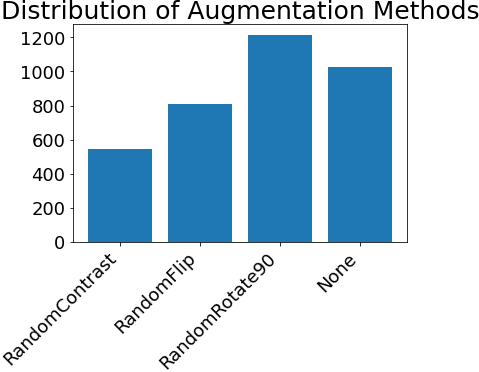
\includegraphics[width=\textwidth]{images/clf-aug-dist.png}
        \caption{Distributions for the classification task data set.}
        \label{fig:clf-augmentation-distribution}
    \end{minipage}
\end{figure}

\subsection{Filtering}\label{subsec:filtering}
Using filters on images can improve the quality of prediction of an algorithm as presented in the initial paper of VGG~\cite{VGG16}.
A preprocessing color correction filter is used in VGG-16 to potentially overcome the issue of having too dark images in the train set that don't represent the production data that is expected.
Hence, when using a pretrained model, in the example of VGG-16 and MobileNet here both are using a base of existing weights~\footnote{
    In the implementation this is done by providing a string value representing the name of the data set that was used to generate the weights, here \path{'imagenet'} weights are used (for more see the documentation of Keras-Applications: \url{https://keras.io/api/applications/}).
}, it is required to use the provided preprocessing method during inference time.
Omitting the method would result in unpredicted input data and the method would respond with poor predictions.
Examples for such preprocessing methods are visualized in \figref{fig:mobilenet-preprocessing} and \figref{fig:vgg-16-preprocessing}.

\begin{figure}[!ht]
    \begin{minipage}{0.45\textwidth}
        \includegraphics[width=\textwidth]{images/mobilenet-preprocessing.eps}
        \caption{Image pre-processed for MobileNet}
        \label{fig:mobilenet-preprocessing}
    \end{minipage}
    \hfill
    \begin{minipage}{0.45\textwidth}
        \includegraphics[width=\textwidth]{images/vgg-16-preprocessing.eps}
        \caption{Resulting image of pre-processing method for VGG-16}
        \label{fig:vgg-16-preprocessing}
    \end{minipage}
\end{figure}

\subsection{Dimensionality Reduction}\label{subsec:dimensionality-reduction}
Sometimes the input data can not be resized, cropped or transformed using simple pixel wise operations.
And sometimes there are too many input features available to use while fitting the desired method, which can cause issues regarding resource and performance constraints.
For this reason a technique called "Dimenionality Reduction" is introduced, that reduces the dimensions of the input data.\\
Let $R: \R^{N_i} \rightarrow \R^{N_o}$ be a reduction function with $N_i$ the number of input features and $N_o$ the number of output features~\footnote{
    Later, in other transformations will be no differentiation between $N_i$ and $N_o$, all inputs are considered to be in the size $N$ where $N$ depends on the transforming method.
}.
For this reason a more sophisticated decision algorithm was applied, \textbf{P}rincipal \textbf{C}omponent \textbf{A}nalysis (PCA).
PCA essentially extracts the most correlating components out of the training images, the principal components, and stores them in a format where the first component is the most correlating one and the last component is the component with the least correlation to others.\footnote{
    For more information, theory and background see~\cite{pca, handsOn}.
}
Let $\PCA_N$ be the PCA containing the $N$ most correlating components of the training data set, then the function $R: \R^{N} \rightarrow \R^N, R\left(\mybold{x^{(m)}}\right) \mapsto \mybold{x^{(m)}}_R$ describes the transformation of an image onto these components, where $\mybold{x^{(m)}}_R$ is the reduced form of $\mybold{x^{(m)}}$.
This gives a great advantage for some of the conventional methods, due to the fact that it is not required to consist of $150528$ parameters.
Unfortunately this results in a changed image that can not be displayed in a proper way, nor processed by a CNN-architecture, this will be discussed in the upcoming chapter.
The following section will give an introduction to algorithms and architectures used to solve the tasks of this paper.
